\section{Result}
This section will look at the results in the form of calculated equations of motion and steady state solutions. Both with and without feedback. The first subsection will deal with a QHO which is measured continuously and without feedback, while the second subsection will add feedback into the scheme.
\subsection{Measurement Without Feedback}
Consider a QHO described by the Hamiltonian in Eq. \eqref{eq:hamiltonian} which is coupled to a thermal bath with temperature $T$. If the oscillator's position quadrature is also continuously measured the evolution of the system can be described by the master equation in Eq. \eqref{eq:masterMeas} using the Lindblad operators mentioned in Sec. \ref{sec:mastereq}. We want to solve for \gls{eom} when measuring for the position quadrature
\begin{align}
    \dt\expval{\xop^2} &= \tr(\xop^2 \dt \dmatrix)\label{eq:x2}, \\
    \dt\expval{\pop^2} &= \tr(\pop^2 \dt \dmatrix)\label{eq:p2},\\
    \dt\expval{\acomm{\xop}{\pop}} &= \tr(\acomm{\xop}{\pop} \dt \dmatrix). \label{eq:xp}
\end{align}
The choice of looking at the second momenta has to do with their relation to the variance and thus the fluctuations of the system. These fluctuations are then related to the energy contained in the oscillator. When looking at feedback control and interesting application is to minimize the energy in the oscillator and, which is thus also an argument for looking at the second momenta.
Solving Eqs. \eqref{eq:x2} to \eqref{eq:xp} yields the following EOM
\begin{align}
    \dt\expval{\xop^2} &= - \gamma \expval{\xop^2} - \frac{1}{m}\expval{\acomm{\xop}{\pop}} + \frac{\gamma \hbar}{m\omega}(\nbar + 1/2),\\
    \dt\expval{\pop^2} &= -\gamma \expval{\pop^2} + m\omega^2 \expval{\acomm{\xop}{\pop}} + \gamma m \omega\hbar (\nbar + 1/2) + \lambda \hbar^2,\\
    \dt\expval{\acomm{\xop}{\pop}} &= -\gamma \expval{\acomm{\xop}{\pop}} + 2 m \omega^2 \expval{\xop^2} - \frac{2}{m} \expval{\pop^2}
\end{align}
for more detailed calculations see App. \ref{app:eom}. Performing a change of variable to make the equations dimensionless
\begin{equation}
    \tilde{x} = \sqrt{\frac{m\omega}{\hbar}} x \quad \text{and} \quad \tilde{p} = \sqrt{\frac{1}{m \omega \hbar}} p ,
\end{equation}
we can solve for the steady state. By introducing the quality factor $Q = \omega / \gamma$ we obtain the steady state solutions
\begin{align}
    \expval{\tilde{x}^2}_\mathrm{ss} &= (\nbar + 1/2) + \frac{\lambda \hbar}{m \omega^2} \frac{2 Q^3}{4Q^2 + 1}, \label{eq:x2ss}\\
    \expval{\tilde{p}^2}_\mathrm{ss} &= (\nbar + 1/2) + \frac{\lambda \hbar}{m \omega^2} \left( Q - \frac{2Q^3}{4Q^2 + 1} \right) \label{eq:p2ss},\\
\end{align}
One interesting aspects of the equations is that both equations have identical terms capturing the thermal aspect of the fluctuations. Another interesting thing is that without measurement the equations are only thermal, which is to be expected. Interestingly, when calculating the energy of the steady state the complicated fraction disappears and we are left with a purely linear term in the quality factor.
\begin{equation}
    E_\mathrm{ss} = \expval{\tilde{H}}_\mathrm{ss} = \frac{\hbar \omega}{2} \left( \expval{\tilde{p}^2} + \expval{\tilde{x}^2} \right) = \hbar\omega (\nbar + 1/2)+ \frac{\lambda \hbar^2}{2 m\omega} Q
    \label{eq:ess}
\end{equation}

\begin{figure}
    \centering
    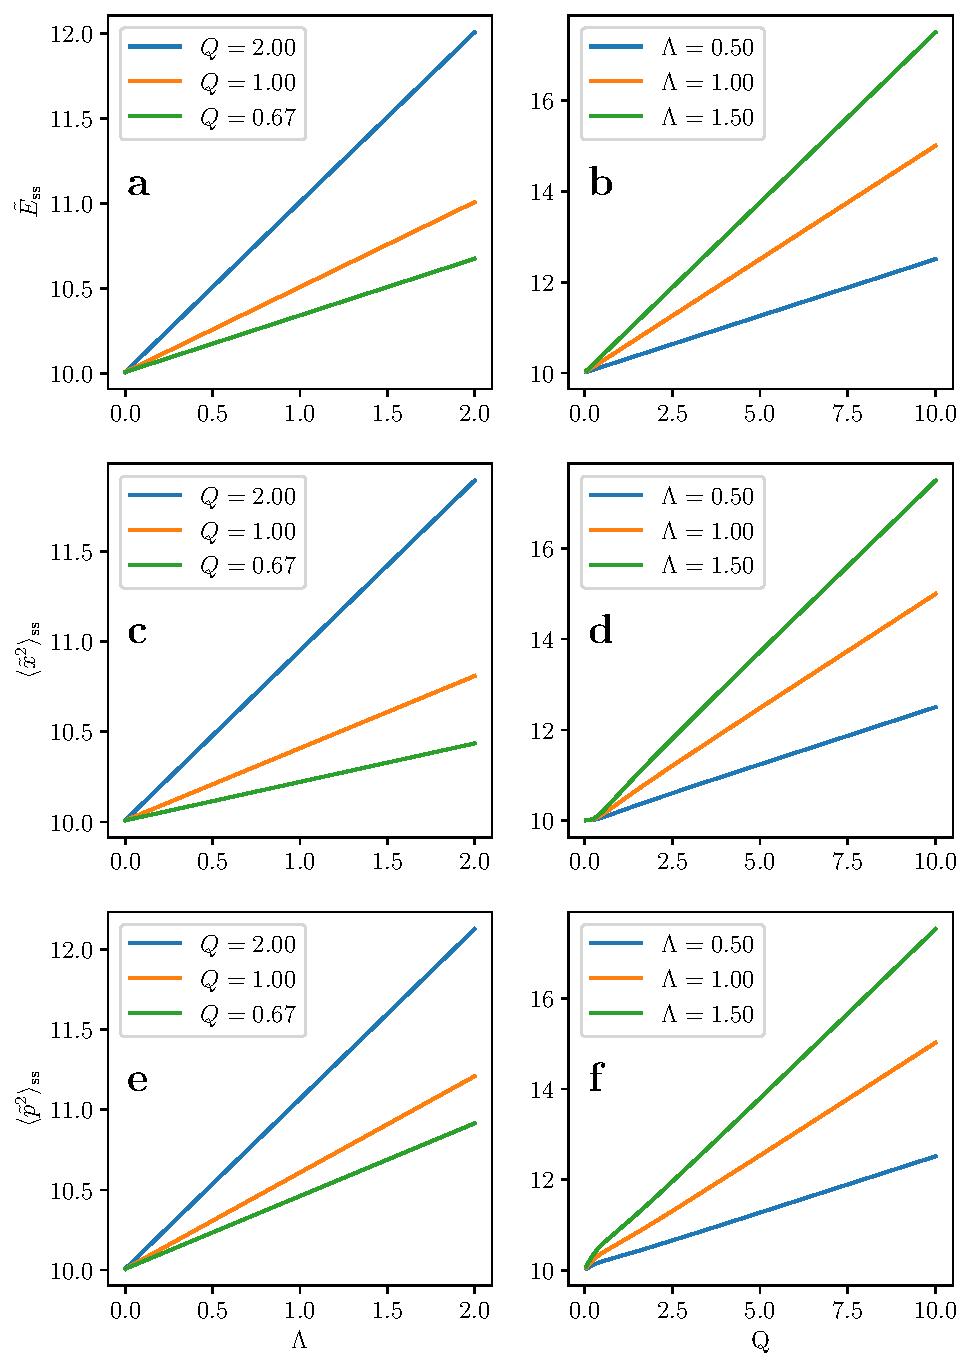
\includegraphics[width=\textwidth]{measurement_result.pdf}
    \caption{ \small The top panels show Eq. \eqref{eq:ess}, the middle panels show Eq. \eqref{eq:x2ss} and the bottom panels show Eq. \eqref{eq:p2ss}. All plots use the parameters $k_\mathrm{B}T = 10$ and $\omega = \hbar = 1$. The left panels are plotted against $\lambda / \omega$ and with three different values for $Q$, while the right panels are plotted against $Q$ and three different values of $\lambda$. }
    \label{fig:steady_state}
\end{figure}

Looking at panels \textbf{a} and \textbf{b} in Fig. \ref{fig:steady_state} one can see that a stronger measurement correlates to the system steady state increasing in energy, as does it for an increasing quality factor. Both also affect the system linearly. Thus, by continuously measuring the system we add energy into it, which make the steady state higher in energy than what the thermal effects from the bath would otherwise place it. That is, if we do not perform any measurement the system would be stable at around $\nbar + 1/2$ which for the parameters used here would give $\expval{\tilde{E}} \approx 10\hbar\omega$

In panels \textbf{d} and \textbf{f} we can see that there is some non-linear behaviour near $Q = 0$. However, due to the approximations made in Sec. \ref{sec:open} we cannot trust the results in the region of a low quality factor. Due to this regime having a relatively high coupling to the environment, and thus the excitations in the environment might not decay fast enough and therefore affect the oscillator. Panels \textbf{c} and \textbf{e} show the linear dependence on $\lambda$ for the second momenta.

Using the same master equation as above we can also solve for the first momenta
\begin{align}
    \dt\expval{\xop} &= \tr(\xop \dt \dmatrix),\\
    \dt\expval{\pop} &= \tr(\pop \dt \dmatrix).
\end{align}
Solving these equations we find 
\begin{align}
    \dt\expval{\xop} &= -\frac{\gamma}{2} \expval{\xop} - \frac{1}{m} \expval{\pop},\\
    \dt\expval{\pop} &= -\frac{\gamma}{2} \expval{\pop} + m\omega^2 \expval{x}.
\end{align}
Then when solving for the steady state we find 
\begin{equation}
    \expval{\xop} = \expval{\pop} = 0. \label{eq:xp0}
\end{equation}
This result also confirms the intuition that for a harmonic oscillator, the system has a steady state around the origin. To check for stability we can rewrite the equation as an eigenvalue problem and solve for the eigenvalues. That is, for the matrix
\begin{equation}
    \mathcal{M} = \begin{pmatrix}
        -\gamma/2 & -1/m \\
        m\omega^2 & -\gamma/2
    \end{pmatrix}
\end{equation}
the eigenvalues are 
\begin{align}
    \lambda_1 &= -\frac{\gamma}{2} - i\omega,\\
    \lambda_2 &= -\frac{\gamma}{2} + i\omega.
\end{align}
Since the real part of the eigenvalues are negative the system is stable.

Eq. \eqref{eq:xp0} also shows that the variance of the system is only dependent on the first momenta, since
\begin{equation}
    \sigma^2_{\hat{A}} = \expval{\hat{A}^2} - \expval{\hat{A}}^2
\end{equation}
for an operator $\hat{A}$. It is also an easy calculation then to show that for temperature $T=0$ and without measurement we have equality in the Heisenberg uncertainty relation, justifying the accuracy of the results, and the approximations made in the derivation of the master equation.

\subsection{Feedback}
We now consider a feedback mechanism on the oscillator described by Eq. \eqref{eq:masterFeed} which is a linear feedback scheme. Solving for the first momenta's EOM we find 
\begin{align}
    \dt\expval{\xop} &= - \left(\frac{\gamma}{2} + \frac{2 \im{f}}{\sqrt{2 m \omega \hbar}} \right)\expval{\xop} - \frac{1}{m} \expval{\pop},\\
    \dt\expval{\pop} &= -\frac{\gamma}{2}\expval{\pop} + \left(\re{f} \sqrt{\frac{2 m \omega}{\hbar}} + m \omega^2 \right) \expval{\xop}.
\end{align}
Choosing $f$ such that
\begin{equation}
    \re{f} = - \sqrt{\frac{m \omega^3 \hbar}{2}} \quad \text{and} \quad \im{f} = -\frac{\gamma\sqrt{m\omega\hbar}}{2\sqrt{2}} \label{eq:reFimF_toZero}
\end{equation}
The system of equations reduces to
\begin{align}
    \dt\expval{\xop} &= - \frac{1}{m} \expval{\pop},\\
    \dt\expval{\pop} &= -\frac{\gamma}{2} \expval{\pop},
\end{align}
which has a steady state solution for $\expval{\pop} = 0$ and any $\expval{\xop}$. To check for stability we can again rewrite the equations as an eigenvalue problem with matrix
\begin{equation}
    \mathcal{M} = 
    \begin{pmatrix}
        - \left(\frac{\gamma}{2} + \frac{2 \im{f}}{\sqrt{2 m \omega \hbar}} \right) & - \frac{1}{m} \\
         \re{f} \sqrt{\frac{2 m \omega}{\hbar}} + m \omega^2 & -\frac{\gamma}{2} &, 
    \end{pmatrix} 
\end{equation}
which has eigenvalues
\begin{equation}
    \varepsilon\pm = \frac{\pm \sqrt{2} \sqrt{ -m^2 \left( 2 \sqrt{2} \re{f} \omega \hbar \sqrt{\frac{m\omega}{\hbar}} + 2 m \omega^3 \hbar - \im{f}^2 \right) } -\sqrt{2} m \im{f} - \gamma m \sqrt{m \omega \hbar} }{ 2 m \sqrt{ m \omega \hbar}}. \label{eq:eigenvalueFirstMomenta}
\end{equation}
Inserting the values of $\re{f}$ and $\im{f}$ from Eq. \eqref{eq:reFimF_toZero} we find the eigenvalues to be $\varepsilon_- = -\gamma /2$ and $\varepsilon_+ = 0$. It is interesting that this choice of $f$ removes all the oscillatory behaviour from the system, which can be seen by the eigenvalues being real. Since one of the eigenvalues are zero the system is also reduced to a one dimensional problem, which is reasonable as the choice of $f$ is such that the system is unaffected by the position quadrature.

\begin{figure}
    \centering
    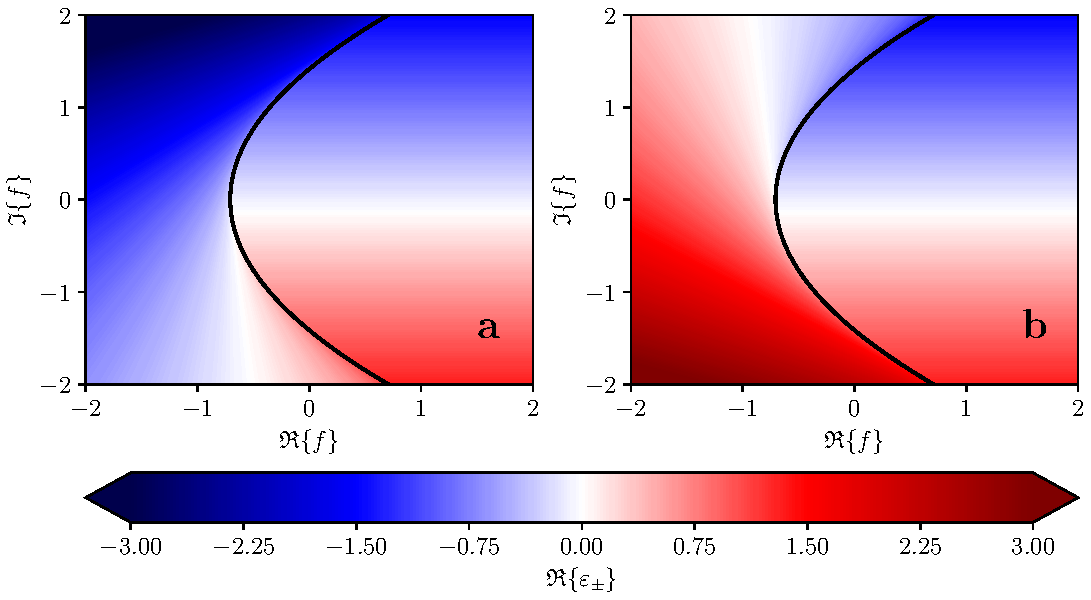
\includegraphics[width=\textwidth]{figures/eigenvalueFirstMomenta.pdf}
    \caption{\small Eq. \eqref{eq:eigenvalueFirstMomenta} plotted as a contour plot against the real and imaginary part of $f$. The parameters used are $m = \omega = \hbar =1$ and $\gamma = 0.2$. Panel \textbf{a} shows $\re{\varepsilon_-}$ and panel \textbf{b} shows $\re{\varepsilon_+}$. The parabola that can be seen in both panels is the points where the first square root in Eq. \eqref{eq:eigenvalueFirstMomenta} is zero. Thus, points to the left of this parabola are real, while points to the right are complex, only the real part is plotted, however.}
    \label{fig:eigenvalueFirstMomenta}
\end{figure}

Looking at Fig. \ref{fig:eigenvalueFirstMomenta} we can see that $\re{\varepsilon_-}$ is mostly negative while $\re{\varepsilon_+}$ is mostly positive for the parameters used in the region closest to the origin. The only part where both eigenvalues are negative is in top right region of the figures. That is, the region where $\im{f} > 0$ and $\re{f} \gtrapprox -1 / \sqrt{2}$. The reason for the approximate is that looking at panel \textbf{b} we can see that line where the eigenvalue is zero has a slant and is not vertical.

Since we can write the solutions as an exponential with the eigenvalues while the coefficients are chosen by the initial condition the value of the eignvalue will determine the behaviour of the system. The consequence of the eigenvalue being negative is that it will make the function decay with time and is thus considered stable. If both eigenvalues are negative the system will decay no matter what the initial conditions are since both terms in the solution will decay. Positive eigenvalues on the other hand will correspond to the system growing with time and will thus be unstable. When one of the eigenvalues is positive and the other is negative the stability of the system will be determined by the initial conditions. That is, the initial condition will determine which eigenvalue will dominate the solution.

Another thing to note is that the eigenvalues are comples to the right of the black parabola in the figure, and thus the solution will have oscillatory motion in this region.

Solving for the EOM for the second momenta we obtain
\begin{align}
    \dt \expval{x^2} &= -\left(\gamma + \frac{4\im{f}}{\sqrt{2 m \omega \hbar}}\right) \expval{x^2} - \frac{1}{m} \expval{\acomm{x}{p}} + \frac{\gamma \hbar}{m \omega} (\nbar + 1/2) - \frac{1}{4\lambda m \omega \hbar} \re{f}^2,\\
    \dt \expval{p^2} &=  -\gamma \expval{p^2} + \left( m\omega^2 + \re{f} \sqrt{\frac{2m \omega}{\hbar}} \right)\expval{\acomm{x}{p}} + \gamma m \omega \hbar (\nbar + 1/2) + \lambda \hbar^2 + \frac{m \omega}{4 \lambda \hbar}\re{f}^2 ,\\
    \dt \expval{\acomm{x}{p}} &= \left(\gamma + \frac{2\im{f}}{\sqrt{2m \omega \hbar}}  \right)\expval{\acomm{x}{p}} + \left(2 m \omega^2 + 2 \sqrt{\frac{2 m \omega}{\hbar}}\re{f} \right) \expval{x^2} - \frac{2}{m} \expval{p^2} - \frac{\re{f} \im{f}}{2 \lambda \hbar}.
\end{align}
We can solve for the steady state by first rewriting the system of equations to a matrix equation $\dt X = \mathcal{A} X + \mathcal{B}$ where
\begin{equation}
    X =
    \begin{pmatrix}
        \expval{\xop^2}\\
        \expval{\pop^2}\\
        \expval{\acomm{\xop}{\pop}}    
    \end{pmatrix}, \quad
    \mathcal{A} = \begin{pmatrix}
        -\left(\gamma + \frac{4\im{f}}{\sqrt{2 m \omega \hbar}}\right) & 0 & -\frac{1}{m} \\
        0 & -\gamma & m\omega^2 + \re{f} \sqrt{\frac{2m \omega}{\hbar}} \\
        2 m \omega^2 + 2 \sqrt{\frac{2 m \omega}{\hbar}}\re{f} & -\frac{2}{m} & -\left(\gamma +\frac{2\im{f}}{\sqrt{2m \omega \hbar}}\right) \label{eq:matrixA}
    \end{pmatrix}
\end{equation}
and
\begin{equation}
    \mathcal{B} = 
    \begin{pmatrix}
        \frac{\gamma \hbar}{m \omega} (\nbar + 1/2) - \frac{\re{f}^2}{4\lambda m \omega \hbar}\\
        \gamma m \omega \hbar (\nbar + 1/2) + \lambda \hbar^2 +\frac{m \omega \re{f}^2}{4 \lambda \hbar}\\
        -\frac{\re{f} \im{f}}{2 \lambda \hbar}
    \end{pmatrix}.
\end{equation}
To then obtain the steady state solutions is then to solve $X_\text{ss} = - \mathcal{A}^{-1} \mathcal{B}$. To do this is we perform the same change of variables as before, in addition to
\begin{equation}
    \tilde{f} = \frac{f}{\omega \sqrt{m \omega \hbar}} , \quad \Lambda = \frac{\lambda \hbar}{m \omega^2}
\end{equation}
The full analytical solutions are not shown here due to the length of the equations.

\begin{figure}
    \centering
    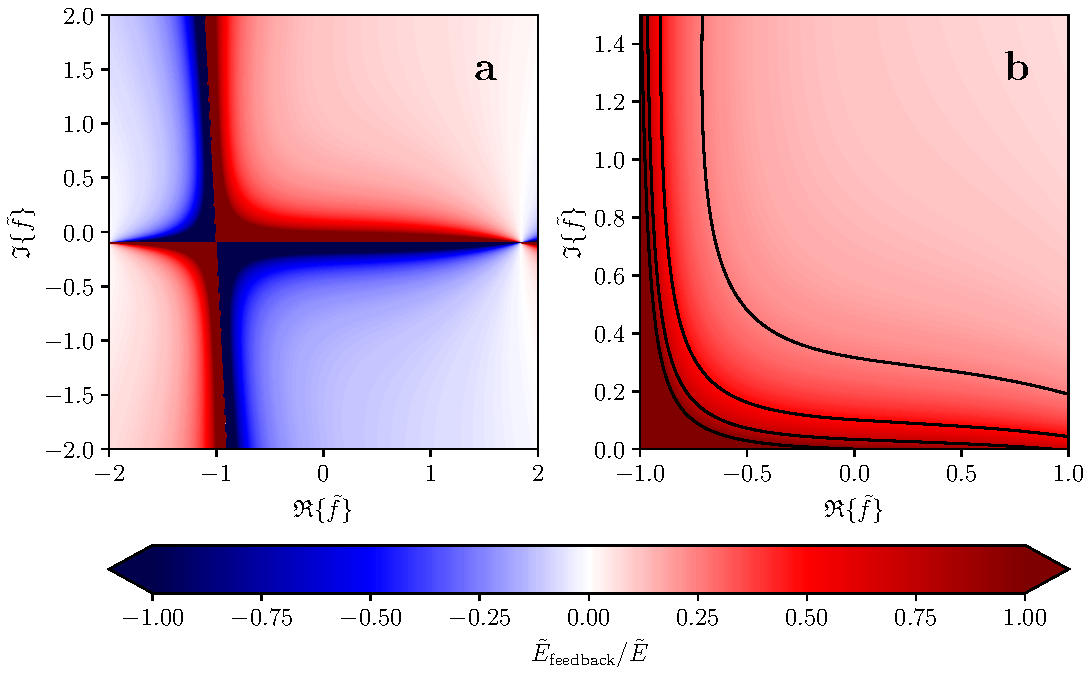
\includegraphics[width=\textwidth]{figures/energyFeedbackRatio.pdf}
    \caption{\small The ratio between the energy with feedback and without plotted as a contour plot against $\re{\tilde{f}}$ and $\im{\tilde{f}}$. The parameters used are $k_\text{B}T = 10$, $Q = 10$, $\Lambda = 2$. Panel \textbf{a} shows a large variation of the parameters. There are divergences in the plot which almost follows a $\left(\re{\tilde{f}} + 1 \right)\im{\tilde{f}} = 1$ curve. Panel \textbf{b} is a zoomed in version of panel \textbf{a} and shows the behaviour of the system in a region where the ratio always is positive.}
    \label{fig:energyFeedbackRatio}
\end{figure}
In Fig. \ref{fig:energyFeedbackRatio} we can see the affect that the feedback has on the energy of the system. Looking at panel \textbf{b} we can see areas which are negative. Since the energy of the system without measurement is constant, as those parameters are frozen, it must be the feedback energy that becomes negative. In the way we have set up the model a negative energy is unreasonable, since a temperature of $T=0$ would correspond to $E =\hbar\omega( 1/2 + \Lambda Q/2)$, which without measurement would mean an energy of $E = \hbar\omega/2$. A possible explantation for the negative energy is that the specific feedback that give rise to this is affecting the system in such a way that at least one of our assumptions is no longer accurate. This could for example be that the system no longer have a physical steady state. Another reason might be that the Markovian approximation no longer holds.

Another interesing aspect of Fig. \ref{fig:energyFeedbackRatio} is that when looking at panel \textbf{b} in conjunction with Eq. \eqref{eq:ess} is that it is possible to cool the system to a lower energy than the thermal energy. Using the same parameters in Eq. \eqref{eq:ess} as are used in the figure we find that the thermal energy is half of the total energy in the system without feedback, and looking at the figure we see that there exist a region which has a ratio of less than $0.5$.


\begin{figure}
    \centering
    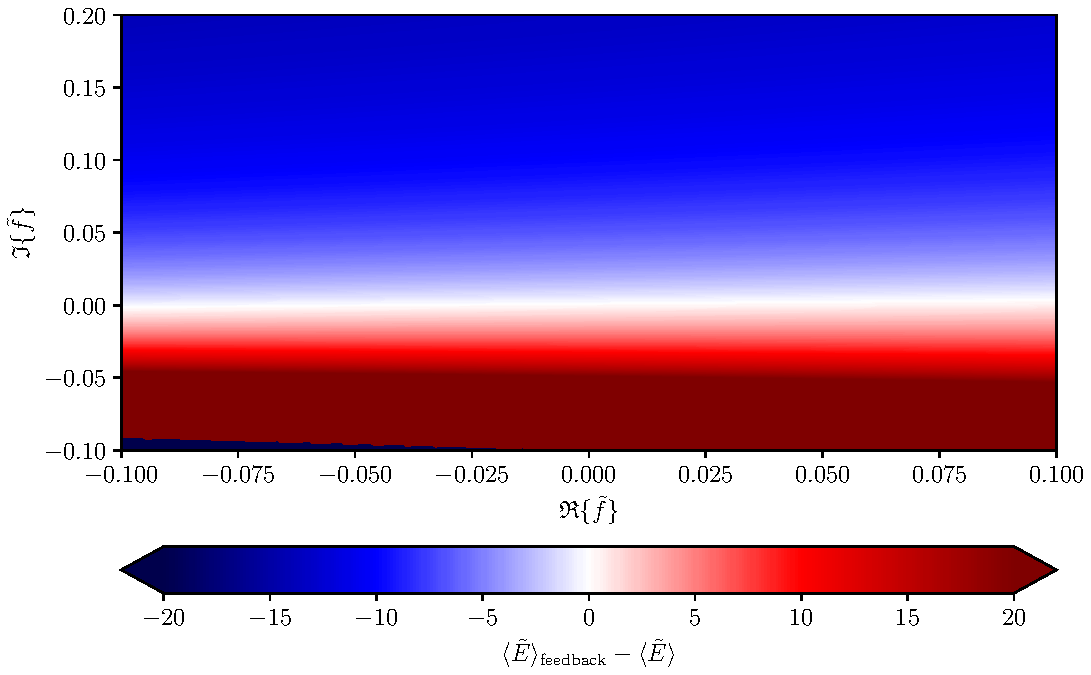
\includegraphics[width=\textwidth]{figures/energyFeedbackDifference.pdf}
    \caption{\small The difference between the energy of the system with feedback plotted and the energy without feedback plotteda against $\re{\tilde{f}}$ and $\im{\tilde{f}}$. The parameters used are $k_\text{B}T = 10$, $Q = 10$, $\Lambda = 2$. The plot is done in a small region around the origin, thus showing the effect a small feedback has on the system. }
    \label{fig:energyFeedbackDifference}
\end{figure}

Using the parameters listed in Fig. \ref{fig:energyFeedbackDifference} the energy without feedback is $\expval{\tilde{E}} \approx 20$ with the thermal part accounting for around $10$ of that. Looking at Fig. \ref{fig:energyFeedbackDifference} it is possible to see that even with a relatively low amount of feedback the system will be cooled to some degree. However, depending on how the feedback is applied it can also make the energy in the system explode which can be seen for $\im{\tilde{f}} < 0$.

\begin{figure}
    \centering
    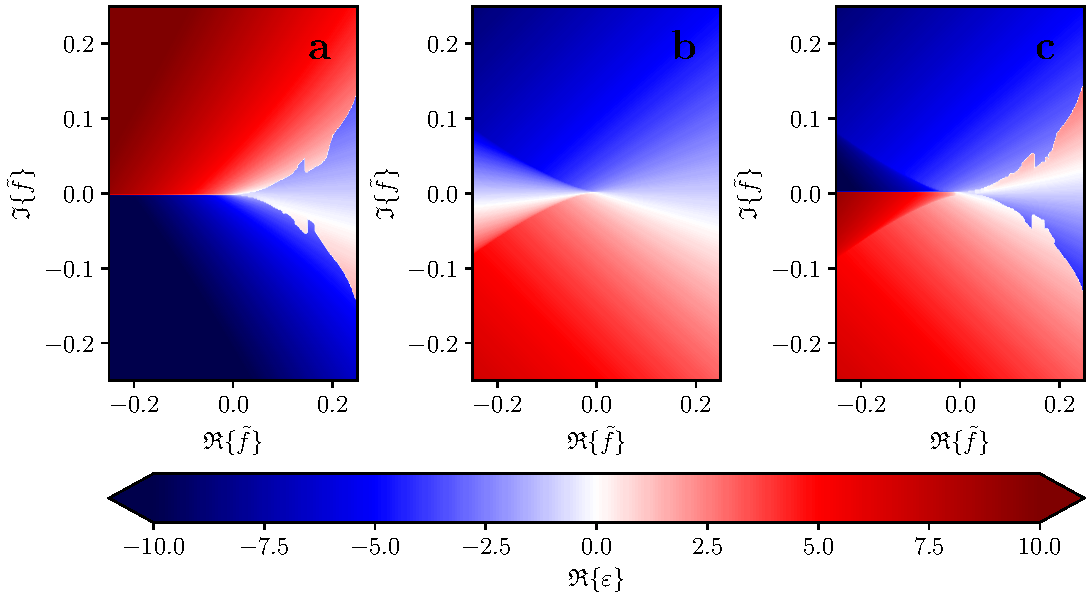
\includegraphics[width=\textwidth]{figures/eigenvaluesSecondMomenta.pdf}
    \caption{The eigenvalues of $\mathcal{A}$ in Eq. \eqref{eq:matrixA} plotted after doing the change of variables as a contour plot against $\re{\tilde{f}}$ and $\im{\tilde{f}}$ using the parameter $Q=10$. Panel \textbf{a}, \textbf{b}, and \textbf{c} show the real part of eigenvalue $\varepsilon_1$, $\varepsilon_2$, and $\varepsilon_3$, respectively.}
    \label{fig:eigenvalueSecondMomenta}
\end{figure}

